\section{Analysis of \DatasetName}
In this section, we first analyze the high-level statistics of our \DatasetName.
Then we analyze the topic modeling and do the qualitative assessment of the properties of \DatasetName.



% \subsection{General Statistics}



% \input{figures/perplexity_distribution}


\paragraph{Perplexity analysis:}
We utilized the pre-trained Llama-2-7B~\cite{llama2} to calculate perplexity scores for 10,000 documents from each dataset.
Lower perplexity scores suggest a stronger resemblance to the types of text corpus used for Llama-2, including Wikipedia and other high-quality sources.
Figure~\ref{fig:quality_metrics}(a) presents the distributions of these scores.
Our findings show that CleanTextSynth has significantly lower average perplexity than LongWordsSubset-A/M.

Additionally, the distribution of TextVisionBlend also aligns closely with that of the high-quality, diverse datasets used for Llama 2 training.
We also observe that the text quality in synthetic datasets, such as CleanTextSynth, is significantly higher than that of real-image subsets like TextScenesHQ.



\begin{figure*}[h!]
    \centering
    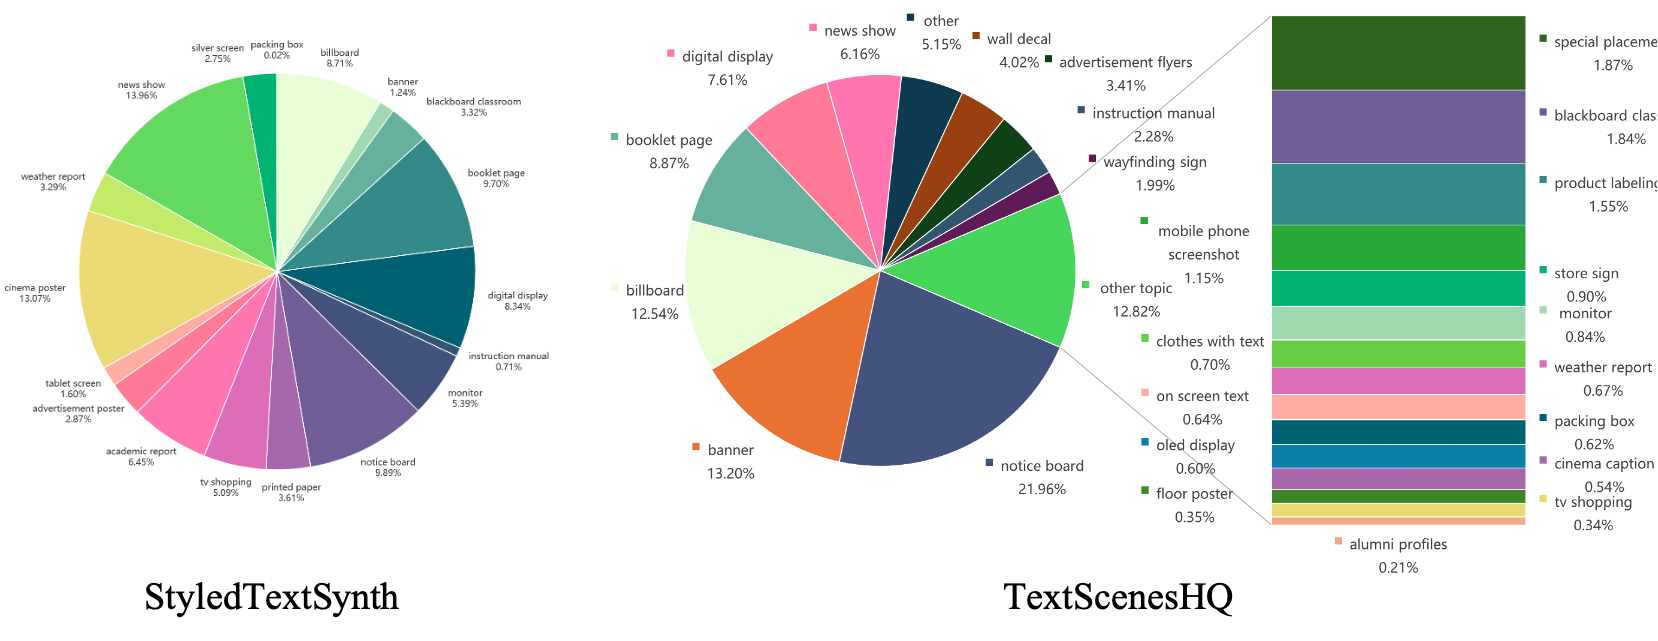
\includegraphics[width=\linewidth]{figures/src/topic_pie_chart.png}
    \vspace{-1em}
    \caption{\textbf{Topic distribution in StyledTextSynth and TextScenesHQ subset, 
    }
    showcasing a diverse range of text-rich topics.
    StyledTextSynth includes carefully selected 18 topics, while TextScenesHQ ultimately contains 26 distinct topics.
    These topics are generated using GPT-4o as a \textbf{world simulator} and then filtered by humans to eliminate overlap while ensuring diversity.
    }
    \label{fig:topic_pie_chart}
\end{figure*}

\begin{figure}[t]
    \centering
    \begin{minipage}[t]{0.47\linewidth}
        \centering
        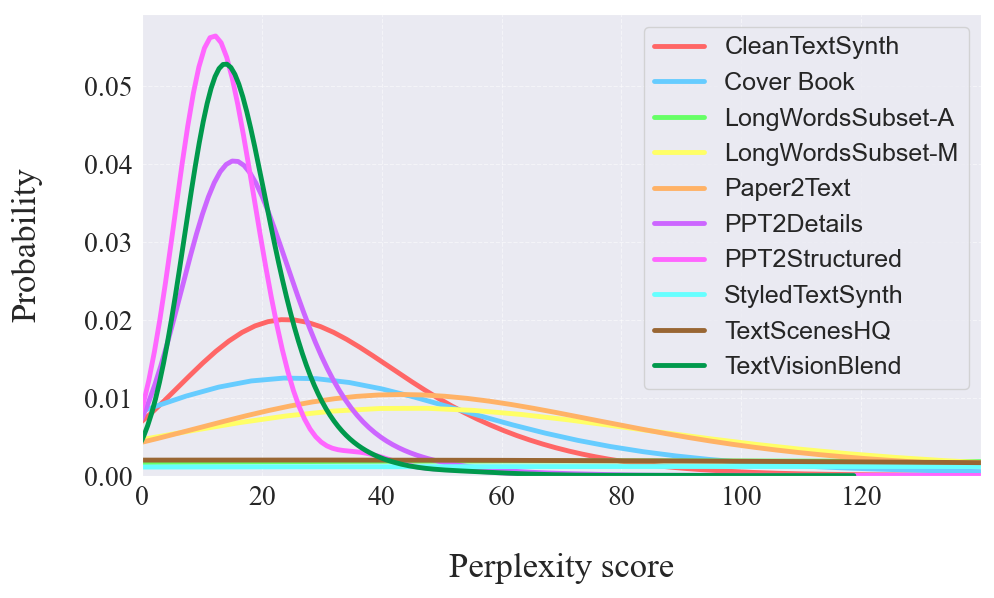
\includegraphics[width=\linewidth]{figures/src/perplexity.png}
        \caption*{\textbf{(a) Perplexity Distribution.} 
        Kernel density estimation comparing; lower perplexity indicates Wikipedia-like content.}
    \end{minipage}%
    \hfill
    \begin{minipage}[t]{0.52\linewidth}
        \centering
        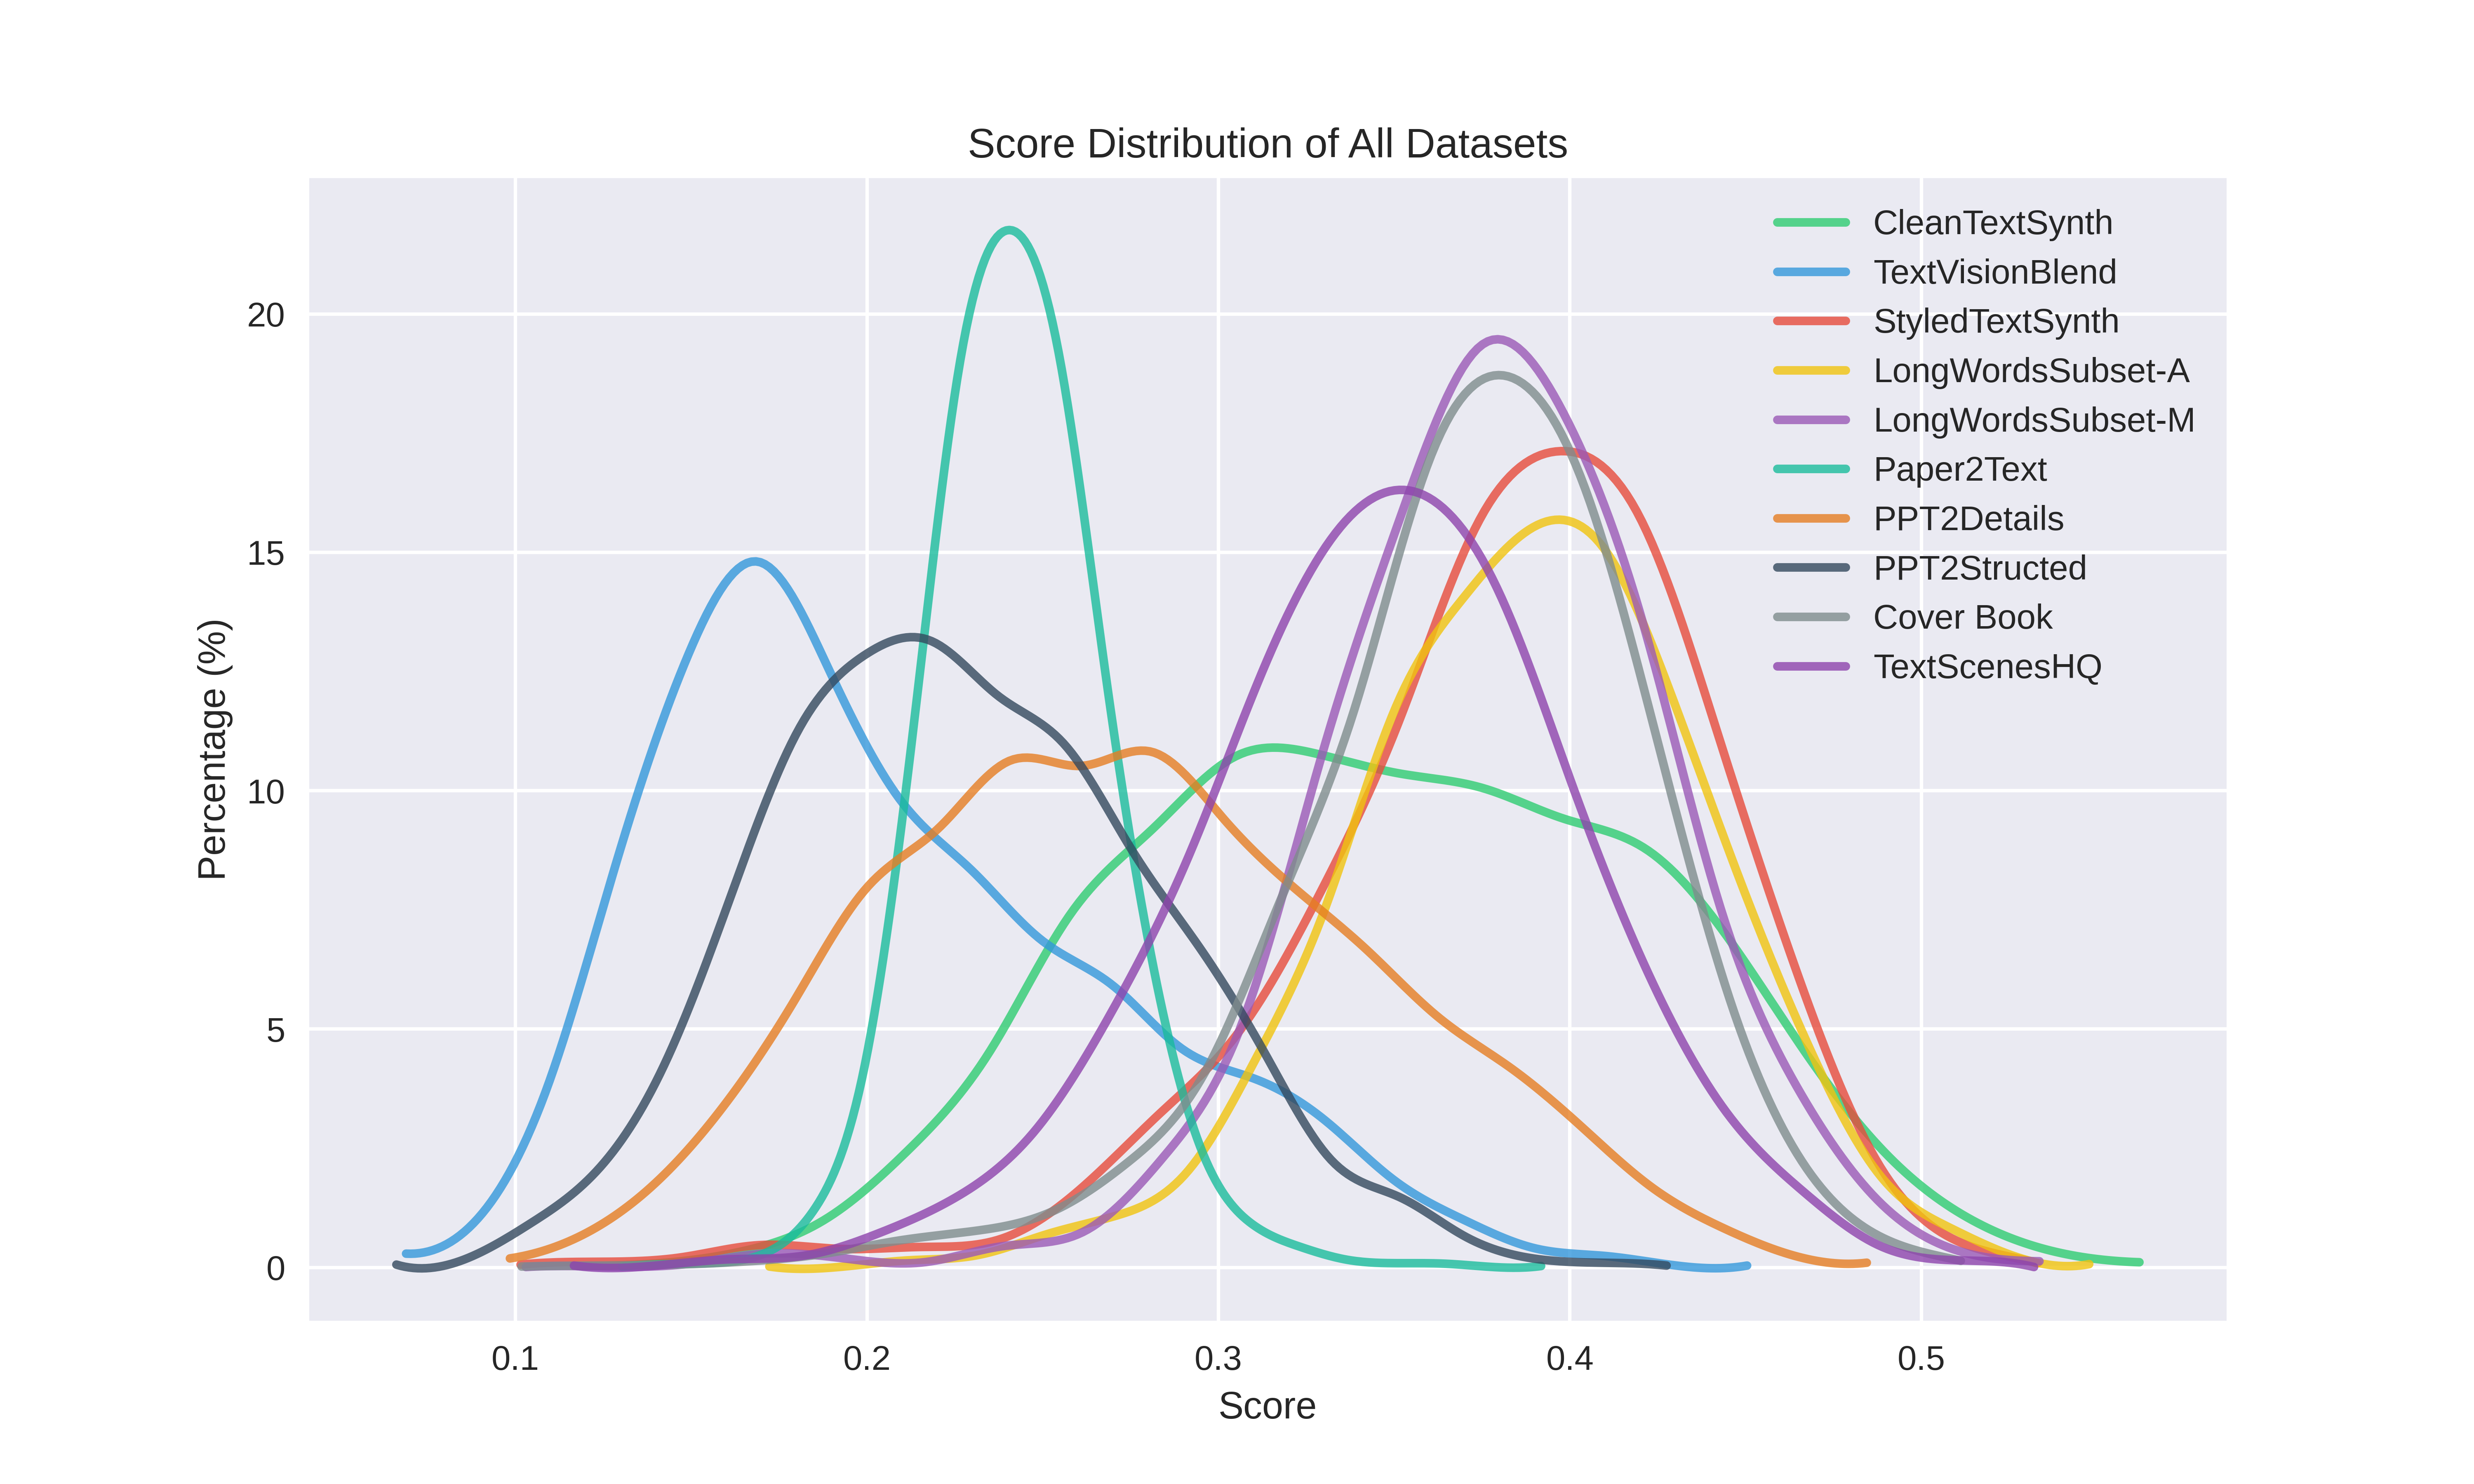
\includegraphics[width=\linewidth]{figures/src/clip_score.png}
        \caption*{\textbf{(b) CLIP Score Distribution.} 
        CLIP score distribution across all \DatasetName~subsets, using 10k random samples each.}
    \end{minipage}
    \caption{\textbf{Linguistic and Visual Quality of \DatasetName.} 
    (a) shows the perplexity distribution of text content, assessing linguistic quality. 
    (b) presents visual-text alignment across subsets.}
    \label{fig:quality_metrics}
\end{figure}


% \begin{figure}[t]
%     \centering
%     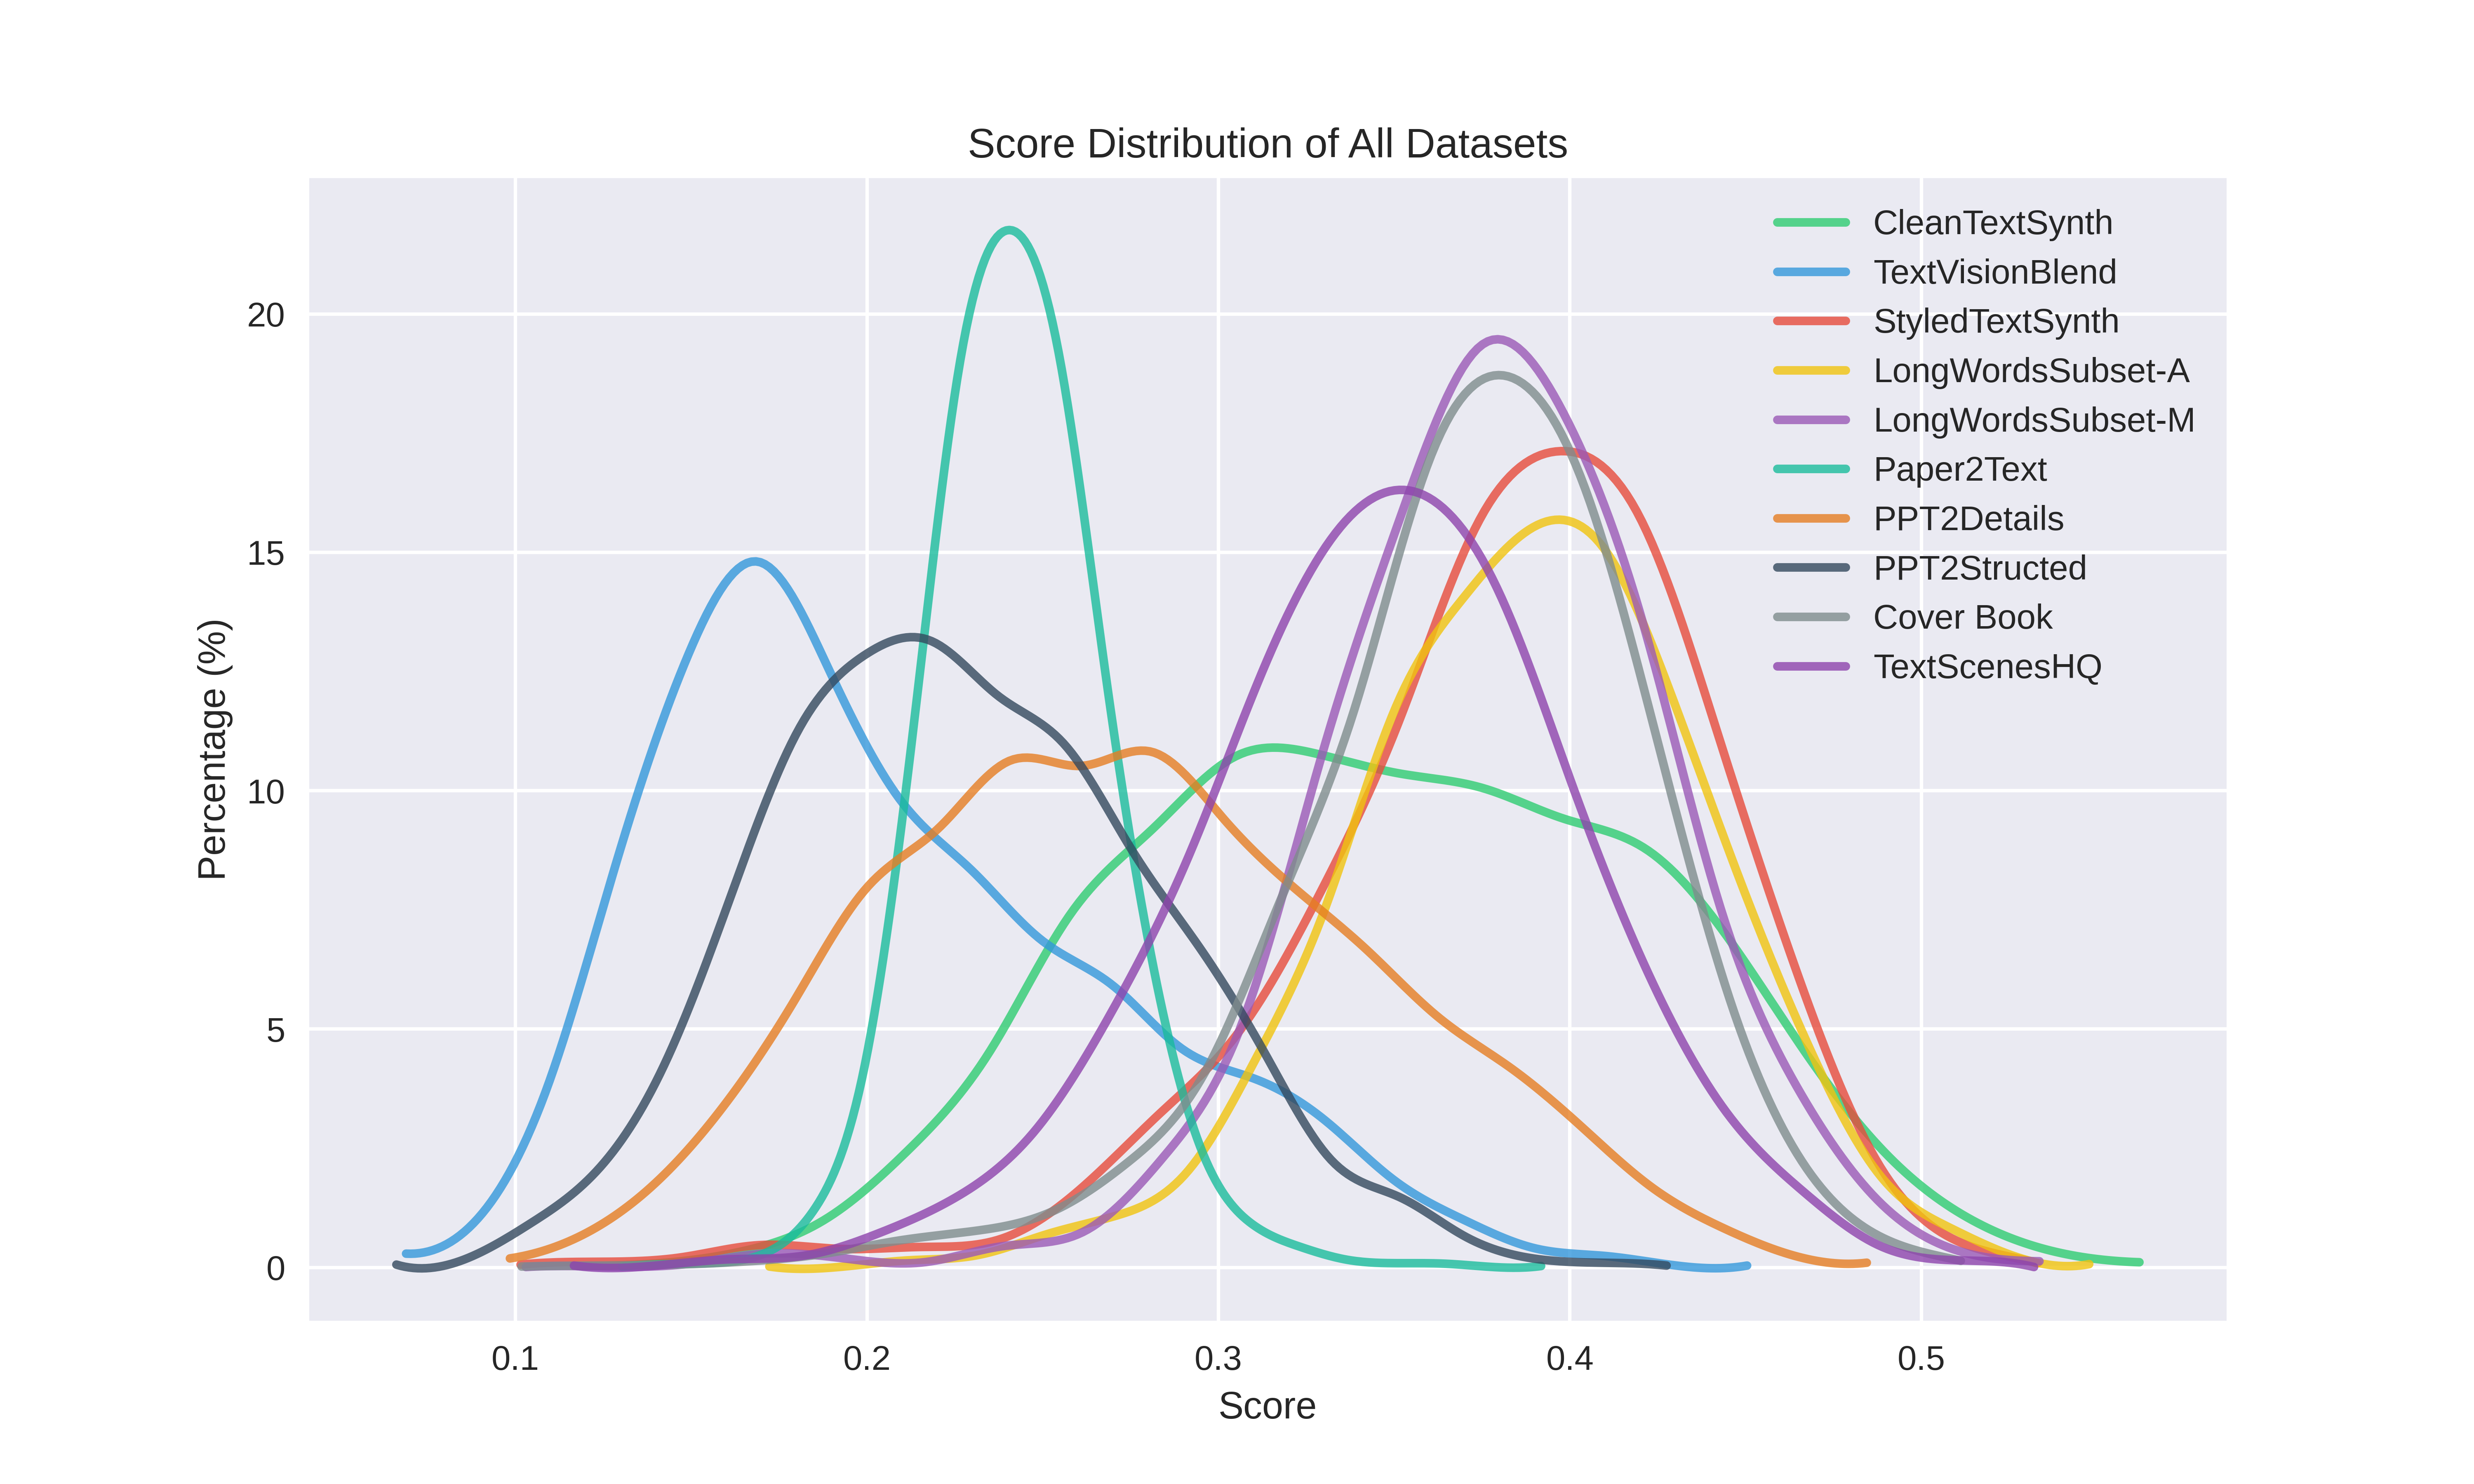
\includegraphics[width=\linewidth]{figures/src/clip_score.png}
%     \caption{
%     \textbf{Clip score distribution over all sub datasets in \DatasetName}.
%     We randomly sample 10k samples for each subset in \DatasetName.
%     }
%     \label{fig:clip score subdataset}
% \end{figure}



\paragraph{Topic Analysis in StyledTextSynth and TextScenesHQ:}
As illustrated in Figure~\ref{fig:topic_pie_chart}, we present an analysis of the topic distribution in the StyledTextSynth and TextScenesHQ datasets.
We additionally highlight the broader topic coverage in real images and find:

\emph{i.} Our dataset encompasses a wide variety of text-rich topics, such as weather reports, banners, TV shopping ads, and monitor displays. This diversity is crucial for maintaining the richness and generalizability of the samples.
\emph{ii.} By leveraging LLMs as world simulators to generate topics, we ensure that most topics are consistent across real and synthetic images, effectively bridging the gap between these two data sources.
\emph{iii.} Some topics generated by the LLM are not suitable for rendering, either due to inherent complexities or limitations in the synthetic generation process. 
These topics are excluded to maintain the quality and feasibility of the dataset.



\begin{figure*}[t]
    \centering
    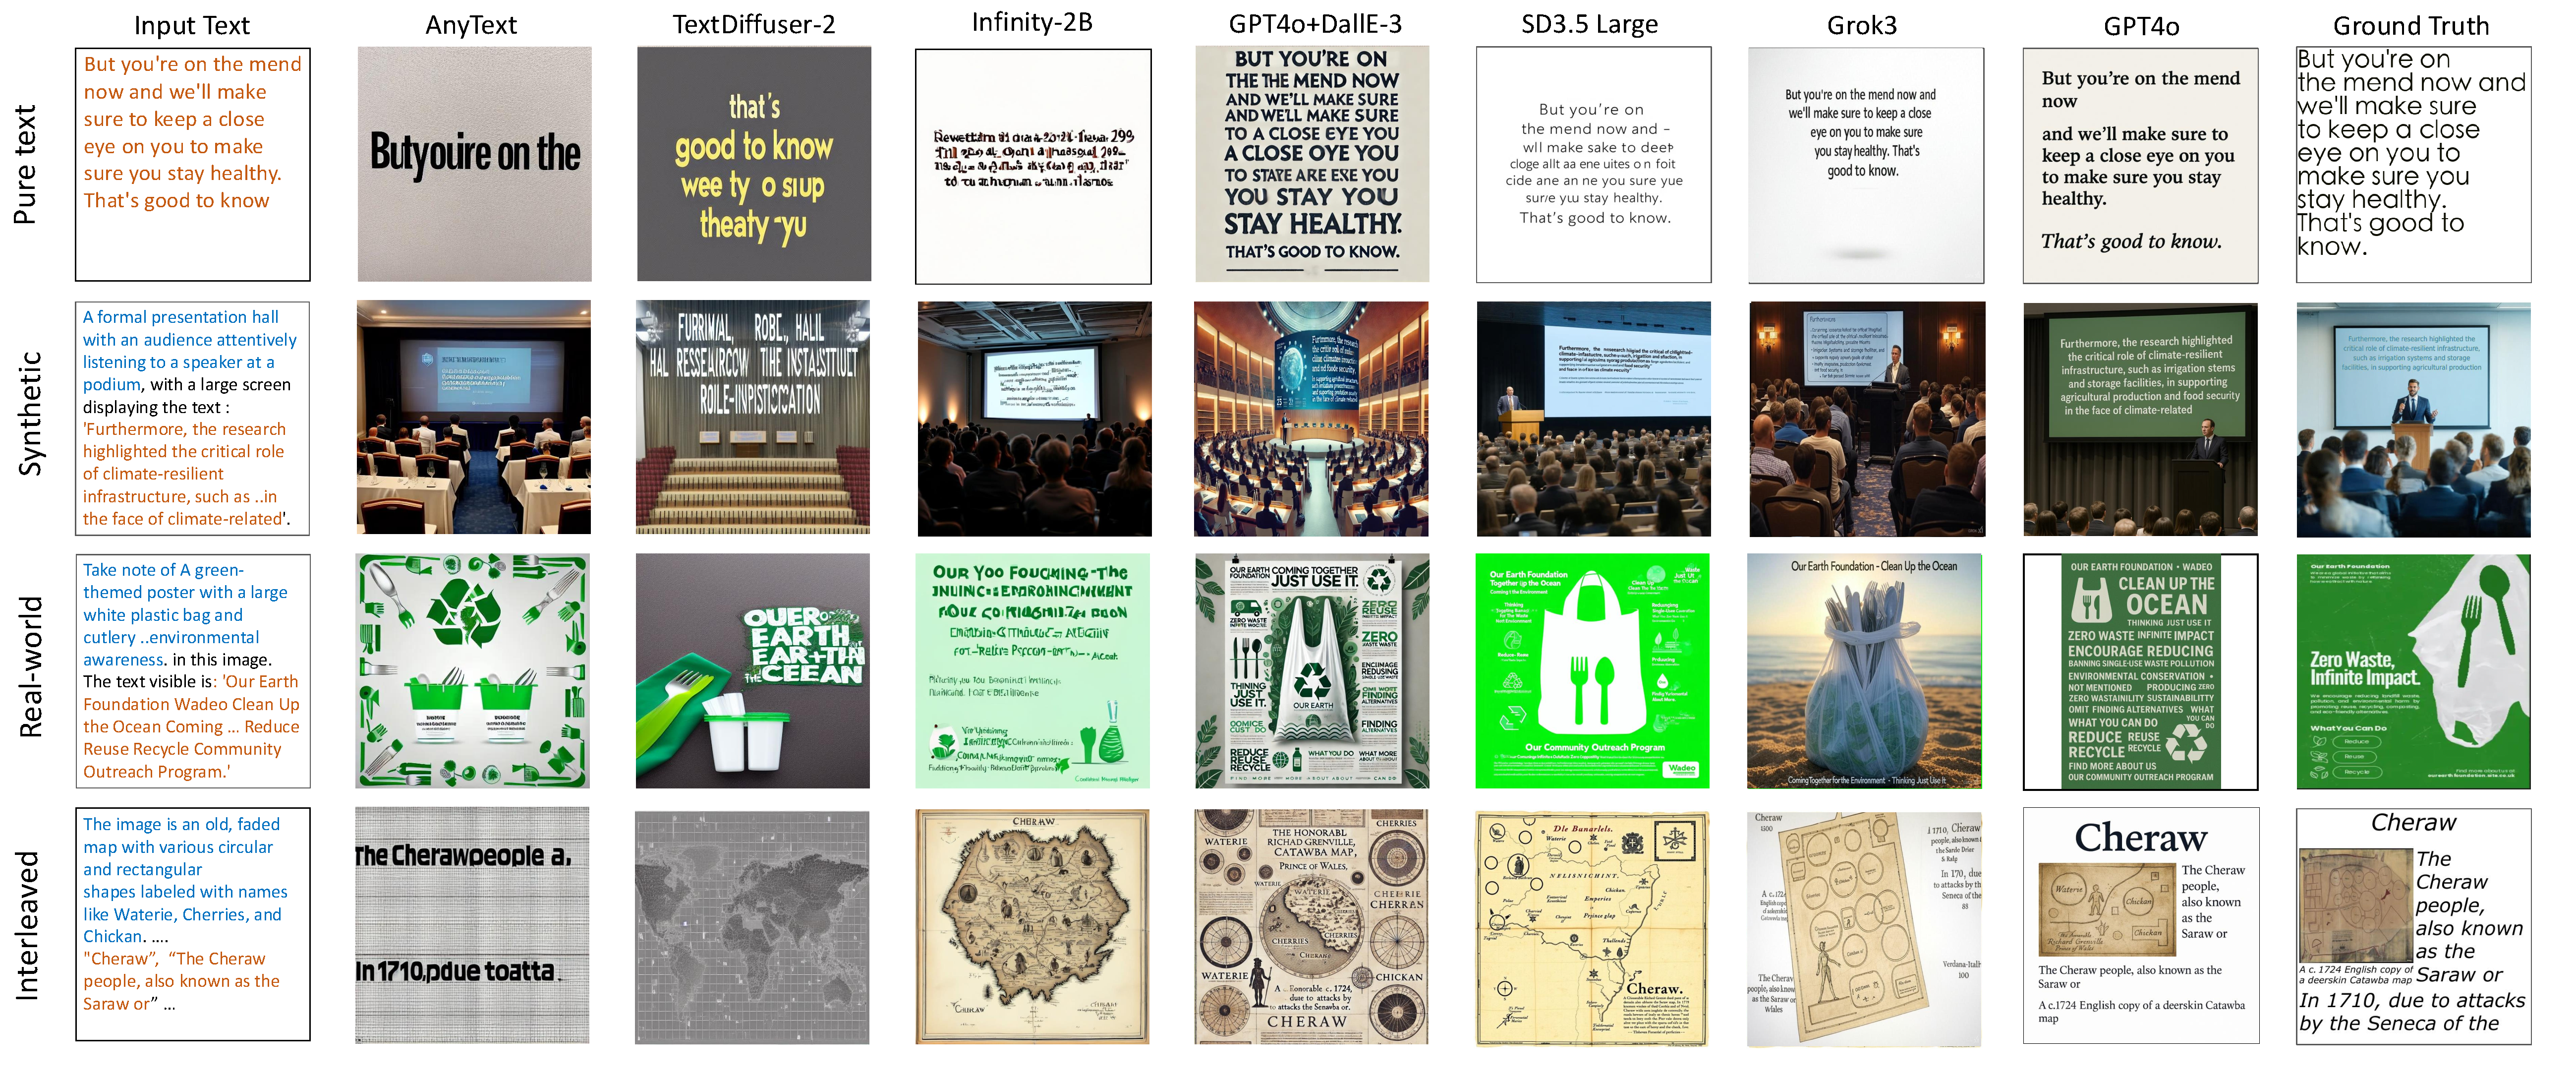
\includegraphics[width=\linewidth]{Appendix/images/text_only_data_v2.pdf}
    \vspace{-1em}
    \caption{
    \textbf{Long text image generation remain challenge for existing model.}
    Existing public methods, such as AnyText~\cite{anytext} and Text Diffuser2~\cite{textdiffuser2}, are capable of rendering short text but struggle with longer sequences. 
    In contrast, GPT4o~\cite{gpt4o} and SD3.5 Large~\cite{sd3} show superior performance, though they still produce inaccuracies such as duplicated words or missing letters when handling extended text.
    For interleaved documents, all methods perform poorly due to their lack of layout planning capabilities.
    The yellow highlights text, while the blue indicates scene descriptions.
    }
    \label{fig:t2i_evaluation}
\end{figure*}


% \input{tables/long_text_generation_comparison}


% \subsection{Qualitative Assessment of Interleaved Samples}

% \subsection{Visual-Linguistic Similarity Assessment}

\paragraph{Visual-Linguistic Similarity Assessment:}
Our dataset primarily consists of English and Chinese, with other languages comprising only 0.3\%.
We assess image-text alignment using CLIP  similarity, where text serves as the query and images as candidates. 
We adopt the ViT-B/32 pretrained on LAION-2B~\cite{openclip}.
As shown in Figure~\ref{fig:quality_metrics}(b), LongWordsSubset-A, -M, and Cover Book yield higher CLIP scores, likely due to the presence of image captions that enhance alignment. 
In contrast, interleaved data shows lower scores, highlighting a challenge for CLIP in parsing visually entangled text layouts. 
Interestingly, Arxiv Paper scores higher than interleaved subsets, suggesting that CLIP retains partial OCR-like capabilities for document-style inputs.




\section{Long Text Image Generation Evaluation}

\begin{figure}
    \centering
    \includegraphics[width=\linewidth]{figures/src/model_visualization.png}
    \caption{
    \textbf{Both Janus-Pro and Lumina-mGPT exhibit significant improvements in text rendering performance when fine-tuned on our \DatasetName}. Notably, while Janus-Pro has baseline support for generating text-rich images, Lumina-mGPT lacks inherent text rendering capabilities.
    }
    \label{fig:trained_model_visualization}
\end{figure}

To evaluate our dataset for long-text image generation, we benchmark both autoregressive (AR) and diffusion models.
Given the limited context capacity of diffusion models, we mainly focus on AR architectures better suited for long-form reasoning.
Concretely, we fine-tune the Chameleon-7B~\cite{chameleon} (with Lumina-mgpt~\cite{lumina_mgpt} decoder) at $512\times512$ resolution and Janus Pro 1B at $1024\times1024$.
For comparison, we also train diffusion model PixArt$\alpha$~\cite{pixarta}.

We benchmark our fine-tuned models against eight state-of-the-art text-to-image generation systems, including open-source baselines (AnyText~\cite{anytext}, PixArt-$\Sigma$~\cite{chen2024pixart}, TextDiffuser-2~\cite{textdiffuser2}, Infinity~\cite{han2024infinity}) and commercial models (DALL·E 3~\cite{dalle3}, SD 3.5 Large~\cite{sd3}, QWEN Image~\cite{qwenimage}. 
We also include closed-source models: GPT-4o (August 2025), Grok3 (May 2025)~\cite{xai2025grok3} and Nano-Banana (September 2025)~\cite{nano_banana_2025}.
For evaluation, we compute image-text similarity using CLIP-ViT-B/32, where higher scores indicate stronger alignment. 
For OCR-based metrics, we use PaddleOCR~\cite{paddleocr} to extract generated text and compare it to ground truth. We report word-level accuracy, F1 score, and character error rate (CER), allowing up to 80\% mismatch tolerance in word-level evaluation.


% 1. PixArt-Alpha~\cite{pixarta}, a state-of-the-art diffusionbased model for text to image generation tasks.
\begin{table*}[t]
\caption{\textbf{Evaluation on \EvalDatasetName across all four subsets.} Metrics include CLIP Score (CS) $\uparrow$, OCR Accuracy (Acc.) $\uparrow$, F1 Score (F1.) $\uparrow$, and Character Error Rate (CER) $\downarrow$. 
Gray rows denote closed-source models. Best and second-best values are highlighted in \textcolor{bestgreen}{green} and \textcolor{secondpink}{pink}, respectively.
$\dag$ means model fine-tuned on our \DatasetName.
Janus Pro 1B~\cite{januspro} use $1024 \times 1024$ resolution and Lumina-mgpt 7B~\cite{lumina_mgpt} adopt $512 \times 512$ resolution.
GPT4o, Dall-E 3 and SD-3.5 Large use  $1024 \times 1024$ resolution and Grok 3 use  $1024 \times 768$ resolution.
}
\centering
\label{tab:eval_all_subsets}
\footnotesize
\setlength{\tabcolsep}{2pt}
\renewcommand{\arraystretch}{1.1}
\resizebox{\linewidth}{!}{
\begin{tabular}{l|x{17}x{18}x{18}x{17}|x{17}x{18}x{18}x{17}|x{17}x{18}x{18}x{17}|x{17}x{18}x{18}x{17}}
\toprule
\textbf{Method} 
& \multicolumn{4}{c|}{\textbf{CleanTextSynth}} 
& \multicolumn{4}{c|}{\textbf{TextVisionBlend}} 
& \multicolumn{4}{c|}{\textbf{StyledTextSynth}} 
& \multicolumn{4}{c}{\textbf{TextScenesHQ}} \\
& CS & Acc & F1 & CER 
& CS & Acc & F1 & CER 
& CS & Acc & F1 & CER 
& CS & Acc & F1 & CER \\
\midrule
AnyText & 0.21 & 0.18 & 0.34 & 0.99 & -& - & - & - & 0.25 & 0.35 & 0.66 & 0.98 & 0.22 & 0.42 & 0.81 & 0.95 \\
TextDiffuser-2 & 0.23 & 1.41 & 2.66 & 0.98 & - & - & - & - & 0.25 & 0.76 & 1.46 & 0.99 & 0.23 & 0.66 & 1.25 & 0.96 \\
PixArt-$\Sigma$ & 0.24 & 0.69 & 1.15 & 0.92 & \cellsecond{0.19} & 2.40 & 1.57 & 0.83 & 0.28 & 0.42 & 0.62 & 0.90 & 0.23 & 0.34 & 0.53 & 0.91 \\
Infinity-2B & 0.24 & 0.11 & 1.93 & 0.88 & 0.20 & 2.98 & 3.44 & 0.83 & 0.27 & 0.80 & 1.42 & 0.93 & 0.23 & 1.06 & 1.74 & 0.88 \\
SD-3.5 Large & \cellsecond{0.28} & 12.0 & 18.2 & 0.84 & 0.18 & 14.55 & 16.25 & 0.88 & 0.28 & 27.21 & 33.86 & 0.73 & 0.24 & 19.03 & 24.45 & 0.73 \\
Qwen Image &-  & - & - & - & 0.18 & \cellbest{81.02} & \cellbest{58.65} & \cellbest{0.57} & \cellbest{0.30} & \cellbest{66.20} & \cellbest{73.92} & \cellbest{0.35} & \cellbest{0.33} & \cellbest{71.82} & \cellbest{68.70} & \cellbest{0.34} \\
\midrule
Janus Pro 1B(1024) & 0.23 & 0.27 & 0.52 & 0.96 & \cellbest{0.22} & 0.76 & 1.31 & 0.94 & 0.27 & 0.06 & 0.12 & 0.98 & 0.27 & 0.25 & 0.48 & 0.98 \\
Janus Pro 1B(1024)$\dag$ & 0.27 & 5.23 & 8.97 & 0.65 & 0.18 & 13.61 & 17.55 & 0.61 & 0.28 & 12.75 & 17.37 & 0.75 & -- & -- & -- & -- \\
% Janus Pro 1B$\dag$ & 0.27 & 5.23 & 8.97 & 0.65 & 0.18 & 13.61 & 17.55 & 0.61 & 0.28 & 12.75 & 17.37 & 0.75 & 0.24 & 0.71 & 1.25 & 0.93 \\
Lumina-mgpt7B(512)& 0.23 & 0.12 & 0.24 & 0.98 & 0.19 & 0.00 & 0.00 & 0.94 & 0.27 & 0.09 & 0.17 & 0.98 & 0.29 & 0.19 & 0.30 & 0.93 \\
Lumina-mgpt7B(512)$\dag$ & {0.27} & {32.90} & {45.93} &{0.35} & 0.16 & {56.61} & {60.18} & {0.26} & 0.27 & {5.43} & {6.71} & {0.71} &{0.27} & {3.83} & {4.65} & {0.78} \\
Lumina-mgpt7B(1024) & 0.24 & 0.32 & 0.45 & 0.97 & 0.18 & 0.03 & 0.05 & 0.95 & 0.27 & 0.13 & 0.21 & 0.97 & 0.28 & 0.22 & 0.35 & 0.92 \\
Lumina-mgpt7B(1024)$\dag$ &\cellbest{0.29}&\cellsecond{48.55}&\cellsecond{59.67}&\cellsecond{0.31}&{0.17}&\cellsecond{65.34}&\cellsecond{70.32}&\cellsecond{0.22}& \cellsecond{0.29}&\cellsecond{27.93}&\cellsecond{20.20}& \cellsecond{0.49} & {0.27} & \cellsecond{6.44} & \cellsecond{9.34} & \cellsecond{0.79} \\
Pixart-$\alpha$ 0.6B(512) &0.25&0.23&0.42&0.98& 0.17 & 0.04 & 0.09 & 0.96 & 0.28 & 0.05 & 0.12 & 0.98 &  0.29 & 0.13 & 0.28 & 0.94 \\
Pixart-$\alpha$ 0.6B(512)$\dag$&\cellsecond{0.28}&39.14&50.24&0.33&0.16&58.21&54.32&0.27& \cellsecond{0.29} & 22.10 & 25.14 & 0.63 & \cellsecond{0.30} & 3.63 & 4.30 & 0.84 \\
\midrule
\rowcolor{grayrow}
Grok3 & {0.28} & 31.08 & 40.81 & 0.44 & 0.17 & 41.54 & 44.22 & 0.57 & {0.29} & 15.82 & 21.4 & 0.73 & 0.32 & 35.07 & 37.94 & {0.57} \\
\rowcolor{grayrow}
DALL·E 3 & -- & -- & -- & -- & {0.19} & 8.38 & 7.94 & 0.93 & {0.29} & 30.58 & 38.25 & 0.78 & {0.34} & 69.26 & 51.63 & 0.67 \\
\rowcolor{grayrow}
Nano Banana & 0.25 & 65.80 & 73.66 & 0.23 & 0.15 & {93.49} & {80.30} & {0.26} &{0.29} & 64.09 & 70.93 & 0.39 & {0.33} & {75.15} & {70.99} & 0.36 \\
\rowcolor{grayrow}
GPT-4o & {0.27} & {60.69} & 74.44 & {0.36} & 0.15 & {91.78} & {82.07} & {0.15} & {0.30} &{77.47} & {80.76} &{0.21} & {0.33} & {82.88} & {78.68} &{0.32} \\
\bottomrule 
\end{tabular}
}
\end{table*}


% \begin{table*}[ht]
% \caption{\textbf{Evaluation on \EvalDatasetName: Interleaved and VeryEasy splits.}\\
% Metrics: CLIP Score (CS), OCR Accuracy (Acc.), F1 score (F1.), and Character Error Rate (CER).}
% \centering
% \label{tab:gen_results_ve_int}
% \footnotesize
% \begin{tabular}{l|x{15}x{23}x{23}x{23}|x{15}x{24}x{24}x{24
% }}
% \toprule
% \textbf{Method} & \multicolumn{4}{c|}{\textbf{CleanTextSynth-Eval}} & \multicolumn{4}{c}{\textbf{TextVisionBlend-Eval}} \\
%  & {CS$\uparrow$} & {OCR (Acc.)$\uparrow$} & {OCR (F1.)$\uparrow$} & {OCR (CER.)$\downarrow$}
%  & {CS$\uparrow$} & {OCR (Acc.)$\uparrow$} & {OCR (F1.)$\uparrow$} & {OCR (CER.)$\downarrow$} \\
% \midrule
% AnyText          & 0.2145 & 0.18 & 0.34 & 0.99 & 0.2501 & 0.35 & 0.66 & 0.98 \\
% TextDiffuser-2   & 0.2260 & 1.41 & 2.66 & 0.98 & 0.2510 & 0.76 & 1.46 & 0.99 \\
% PixArt-$\Sigma$  & 0.2381 & 0.69 & 1.15 & 0.92 & 0.2764 & 0.42 & 0.62 & 0.90 \\
% Infinity-2B      & 0.2429 & 0.11 & 1.93 & 0.88 & 0.2727 & 0.80 & 1.42 & 0.93 \\
% Grok3            & \bf 0.2848 & 31.08 & 40.81 & 0.44 & 0.2854 & 15.82 & 21.40 & 0.73 \\
% DALL·E 3         & -- & -- & -- & -- & 0.2938 & 30.58 & 38.25 & 0.78 \\
% SD-3.5 Large     & 0.2776 & 12.00 & 18.20 & 0.84 &  0.2849 & 27.21 & 33.86 & 0.73 \\
% GPT-4o           & 0.2744 & \bf 60.69 & \bf 74.44 & \bf 0.36 & \bf 0.2968 & \bf 77.47 & \bf 80.76 &\bf  0.21 \\
% \midrule
% Chameleon       & 0.2316 & 0.12 & 0.24 & 0.98 &  0.1929 & 0 & 0 & 0.94 \\
% Chameleon*        & 0.2651 & 32.90 & 45.93 & 0.35 &  0.1603 & 56.61 & 60.18 & 0.26 \\

% \bottomrule
% \end{tabular}
% \end{table*}



\paragraph{Text-to-Image Generation Visualization:}
To provide a clearer understanding, we present visual comparisons in Figure~\ref{fig:t2i_evaluation}.
Our observations highlight that previous open-source text-to-image generation methods beyond SD3.5 Large struggle with rendering dense text. 
For instance, AnyText renders only a handful of words, while Text Diffuser 2 captures only part of the text.
In contrast, GPT-4 demonstrates the best performance in text rendering. 
These results underscore that dense-text image generation remains a challenging task for current models.
Furthermore, we show the base model finetuned on our DatasetName in Figure~\ref{fig:trained_model_visualization}.
It is clear that base model often fail to understand text prompt without text rendering ability.
The model trained with our dataset highly improving text rendering ability over all subsets even very hard real images.


\paragraph{Performance Comparison on All Subsets.}
Table~\ref{tab:eval_all_subsets} shows quantitative results for \EvalDatasetName:

\emph{i.} Models pretrained on our dataset exhibit significant improvements across all evaluation subsets, validating the effectiveness of long-text-focused data. 
\emph{ii.}CleanTextSynth and TextVisionBlend are relatively easier to learn: for instance, Lumina-mgpt and Pixart surpasses GPT-4o in CER on CleanTextSynth, indicating strong capabilities in pure text rendering. Meanwhile, lower CLIP alignment on TextVisionBlend suggests that its synthetic interleaved format remains underrepresented in training of CLIP, posing challenges for existing vision-language models. 
\emph{iii.}
In StyledTextSynth, \textbf{small font sizes make resolution a critical factor, where the tokenizer becomes a performance bottleneck}.
For example, Janus Pro 1B outperform Lumina-mgpt 7B with higher resolution.
% We further discuss this in the supplementary. 
\emph{iv.}
TextScenesHQ remains the most challenging subset due to its diverse topics and complex layouts, requiring \textbf{both accurate prompt understanding and structured generation}. Even under such complexity, our pretrained model achieves a 3.7\% gain in OCR accuracy, underscoring the value of diversity data for enhancing long-text image generation.
\emph{v.}
TextDiffuser2 is pretrained on Marion10M~\cite{textdiffuser2}, which is larger in scale than our \DatasetName. 
Nevertheless, both AR and diffusion models trained on our dataset outperform TextDiffuser2 by a clear margin. 
This highlights that \textbf{\DatasetName fills a critical gap by providing realistic, layout-rich, and semantically diverse text-image pairs missing from existing benchmarks}. 
